\section{Experimental Results}
\label{sec:experiments}

\subsection{Experimental Setup}


In this milestone report, we show experimental results when we apply KNN method to sequences of CPU usage measurements data.
We used Samsung Galaxy S device on which Android 2.3 Gingerbread is running, and Netflix application was used for collecting CPU usage statistics.
10 movies are selected from \term{Popular on Netflix} section of Netflix website and selected movies are shown in Table \ref{tab:movies}.
CPU statistics of selected movies were captured by recording CPU statistics in 1-second and 5-second intervals using the native UNIX command, \term{top}, while playing the first 30 minutes of each movie. 
The measurement was repeated 5 times for each movie.
Measurement results of two selected movies are previously shown in Figure \ref{fig:preliminaries}.

\begin{table}[h!]
\begin{center}
\begin{tabular}{|c|l|c|l|}
\hline
ID & Movie Title & ID & Movie Title \\ 
\hline
1 & Transformers: Dark of the Moon 		& 6 & Super 8\\
2 & Thor								& 7 & Mean Girls 2 \\
3 & Hachi: A Dog's Tale 					& 8 & Captain America \\
4 & The True Story of Puss 'n Boots 		& 9 &  Snatch \\
5 & Wallace \& Gromit: Loaf and Death 		& 10 & No Strings Attached \\
\hline
\end{tabular}
\end{center}
\caption{Selected Movies}
\label{tab:movies}
\end{table}

\subsection{Fast Subsequence Matching Algorithm Results}
Query subsequences are chosen from a 30-min length sequence with varying starting index and length. At every 60 second interval, the subsequencee are selectd with length, $l =$ [180, 240, 300, 600, 900, and 1200] (3, 4, 5, 10, 15, 20 minutes). For each selected subsequence, various lengths of Discrete Fourier Transform window are applied to find better performance. The DFT window with length, $w=$ [50, 100, 150, 200, 300], are applied to extract the two lowest Fourier coefficient ($f=2$). The DFT window length affects the performance of the matching algorithm. If the length of the DFT window is too short, then DFT procedure will result in high noise sensitivity. Otherwise, the DFT procedure results in over-smoothing of the data.

The performance of the matching algorithm is measured by the rate of the number of correct predictions to the number of total queries.
\begin{equation}
R_{succ} = \frac{\#\: of \:correct\: predictions}{\# \:of\: total \:queries}
\end{equation}

The Table \ref{tab:succ_table} shows the success rate of the matching algorithm with varying sequence length and varying DFT window size. It's obvious that the success rate increases as the length of query sequences goes large. As shown in the Table \ref{tab:succ_table}, the success rate increases as the sequence length increases when the size of DFT window is fixed. With the collected movie sequences, our matching scheme gives the best prediction performance when the DFT window length is 200. However, it is impossible to apply DFT procedure with the window lenght 200 to query sequences that are shorter than DFT window length. Those entries in the Table are marked as non-applicable. 

\begin{table}[h!]
\begin{center}
\begin{tabular}{|c|| >{\centering} p{1cm}| >{\centering} p{1cm}| >{\centering}p{1cm}| >{\centering}p{1cm}| >{\centering}p{1cm} |}
\hline
Seq Len ($l$) \textbackslash FFT Len ($w$)& 50 & 100 & 150 & 200 & 300
\tabularnewline
\hline
180 & 0.46 & 0.54 & 0.62 & N/A & N/A
\tabularnewline
240 & 0.475 & 0.585 & 0.64 & 0.655 & N/A
\tabularnewline
300 & 0.52 & 0.595 & 0.665 & 0.65 & 0.69
\tabularnewline
600 & 0.705 & 0.69 & 0.75 & 0.747 & 0.74
\tabularnewline
900 & 0.726 & 0.7428 & 0.8 & 0.791 & 0.72
\tabularnewline
1200 & 0.78 & 0.755 & 0.7875 & 0.814 & 0.74
\tabularnewline
\hline
\end{tabular}
\end{center}
\caption{Selected Movies}
\label{tab:succ_table}
\end{table}

The fast subsequence matching algorithm provides the result very fast in short execution time with considerable accuracy over 70\% when the DFT window length is 200. This efficiency comes from the fact that the algorithm exploits only lowest two frequencies ($f=2$) of (sub-)sequences extracted by DFT to predict the title of the movie. However, the efficiency in the execution time compromises the certainty of our prediction. 

\subsection{KNN Experiment Results}

For each movie, one of five CPU usage sequence is selected as test data and the rest four sequences are considered as training data set. 
The length of subsequence varying from 60 seconds to 360 seconds is set and each test and training data is divided based on the subsequence length as described in \ref{sec:knn}.
When dividing sequence data, we adopt a concept of sliding window which moves by 1 step size.
Each data sequence consists of $360$ measurement points, and therefore $(360 - subsequence\_length + 1)$ subsequences are generated from the data sequence. 

After building up test data set and training data set by generating subsequences, we apply KNN method in order to classify each subsequence of test data based on training data set. 
In this experiment, $k$ value is set to 3 for the simplicity.
The accuracy of classification according to the length of subsequence is shown in Figure \ref{fig:experiment_knn}.
The accuracy is low as 46$\%$ when subsequence length is set to 60-second.
However, the accuracy increases up to 88$\%$ when subsequence is set to 180-second.
The experimental result shows that given 10 movies and CPU usage statistics of 150 seconds, our side channel attack correctly predicts which movie a user is watching at the accuracy of higher than 80$\%$.

\begin{figure}[!h]
\centering
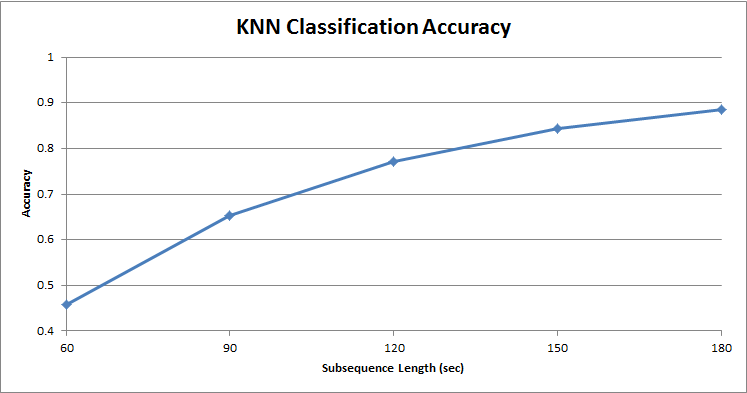
\includegraphics[scale=0.50]{Figures/experiment_knn}
\caption{KNN Classification Accuracy}
\label{fig:experiment_knn}
\vspace{-5mm}
\end{figure}